% per compilarlo "xelatex tesi" PER 2 VOLTE!

% QUESTO PEZZO NON DOVREBBE ESSERE MODIFICATO

\documentclass[12pt,a4paper,oneside,openright]{book}
\usepackage{packages} % inserisce tutti le macro necessarie per il 
                        % funzionamento
\usepackage{frontesp} % modificare questo file per i diplomi e se si ha
                        % un solo correlatore

% LE FIGURE VANNO INSERITE CON ``\includegraphics[width=xxxcm]{file}'' 
% SENZA ESTENSIONE ALTRIMENTI NON SI RIESCE AD OTTENERE IL PDF!!!
% per convertire le figure (ps o eps) in PDF usare 
% epstopdf --outfile=pippo.pdf pippo.ps


\setstretch{1.3}  %interlinea, mettere 1 per singola da usarsi per le bozze!!!

\begin{document}

% DA QUI INIZIA LA PARTE DA MODIFICARE PER INSERIRE IL PROPRIO LAVORO

\title{Questo\\[5mm] \`e il titolo}
\providecommand{\autore}{PINCO PALLINO}                        %candidato
\providecommand{\principaladviser}{Chiar.mo Prof.~A. TIZIO}  %relatore
\providecommand{\firstreader}{Chiar.mo Prof.~P. CAIO}            %correlatore
\providecommand{\secondreader}{Chiar.mo~Prof. R. SEMPRONIO}          %correlatore
\providecommand{\annoacc}{1998--99}
\providecommand{\corso}{\uppercase{Elettronica}} % corso di laurea in ??



% genera la prima pagina

\titlep

% indica l'inizio della parte introduttiva
\frontmatter

   \vspace*{10pc}
\thispagestyle{plain}

\begin{flushright}
\sl

Ai mie genitori\\
e a Giovanna

\end{flushright}
\par\vfill\par

   \tableofcontents
   \listoffigures
   \listoftables
%   \listofalgorithms

\clearpage

% indica l'inizio della parte centrale
\mainmatter
      \chapter*{Introduzione}
\markboth{Introduzione}{Introduzione}
\addcontentsline{toc}{chapter}{Introduzione}


2 paginette giusto per spiegare.

Si noti che questo capitolo viene ottenuto in maniera differente
dagli altri. In particolare non viene numerato.

2 paginette giusto per spiegare.

Si noti che questo capitolo viene ottenuto in maniera differente
dagli altri. In particolare non viene numerato.

2 paginette giusto per spiegare.

Si noti che questo capitolo viene ottenuto in maniera differente
dagli altri. In particolare non viene numerato.

2 paginette giusto per spiegare.

Si noti che questo capitolo viene ottenuto in maniera differente
dagli altri. In particolare non viene numerato.

2 paginette giusto per spiegare.

Si noti che questo capitolo viene ottenuto in maniera differente
dagli altri. In particolare non viene numerato.

2 paginette giusto per spiegare.

Si noti che questo capitolo viene ottenuto in maniera differente
dagli altri. In particolare non viene numerato.

2 paginette giusto per spiegare.

Si noti che questo capitolo viene ottenuto in maniera differente
dagli altri. In particolare non viene numerato.

2 paginette giusto per spiegare.

Si noti che questo capitolo viene ottenuto in maniera differente
dagli altri. In particolare non viene numerato.

2 paginette giusto per spiegare.

Si noti che questo capitolo viene ottenuto in maniera differente
dagli altri. In particolare non viene numerato.


2 paginette giusto per spiegare.

Si noti che questo capitolo viene ottenuto in maniera differente
dagli altri. In particolare non viene numerato.

2 paginette giusto per spiegare.

Si noti che questo capitolo viene ottenuto in maniera differente
dagli altri. In particolare non viene numerato.

2 paginette giusto per spiegare.

Si noti che questo capitolo viene ottenuto in maniera differente
dagli altri. In particolare non viene numerato.
 % attenzione! guardare introd.tex per vedere come e' fatto
      \chapter{File di Esempio}
   Questo 
   file vuole solo essere un esempio di
   \LaTeX2, guardate il sorgente se volete capire come \`e fatto.

   Se inoltre volete capire come mai per scrivere ``è'' ho usato quello strano
   \emph{accrocchio} passate alla sezione~\ref{accenti}, notate inoltre
   che andare a capo due volte di seguito mi genera un nuovo paragrafo.
   Notate che l'\emph{indentatura} che sto usando \`e solo per semplicit\`a.

\section{Grassetto, Italico e amenit\`a varie}
   \`E banale ottenerli (a differenza della ``e'' maiuscola e
   accentata quando usate qualcosa di diverso dal \LaTeX2),
   gi\`a che ci siamo potete anche vedere come si
   ottiene una lista e un nota a pi\`e di pagina:
   \begin{itemize}
   \item \textbf{Grassetto}
   \item \emph{Italico}
   \item \textsc{Maiuscoletto}
   \item \texttt{Macchina da Scrivere}\footnote{In genere \`e conveniente non
                 abusare troppo di questo, visto che \`e gestito male nei rientri a capo.}
   \end{itemize}
\section{Tabelle}

   Per spaventarvi subito guardate un po' come si ottiene la tabella~\ref{miatabella}.
   \begin{table}[h!]
    \centering
    \begin{tabular}{|l|c|c|}
    \hline
    Oggetto & Costo & peso \\
    \hline
    \hline
    Pere    & 123   & 345  \\
    \hline
    Mele    & 234   & 56   \\
    \hline
    \end{tabular}
    \caption{Tabella di esempio\label{miatabella}}
   \end{table}

\section{Figure}
   Molto pi\`u semplice inserire la figura~\ref{miafigura}
   generata usando \texttt{xfig} (ottimo programma
   per fare disegni da inserire in relazioni/tesi). 
   \begin{figure}
   \centering
   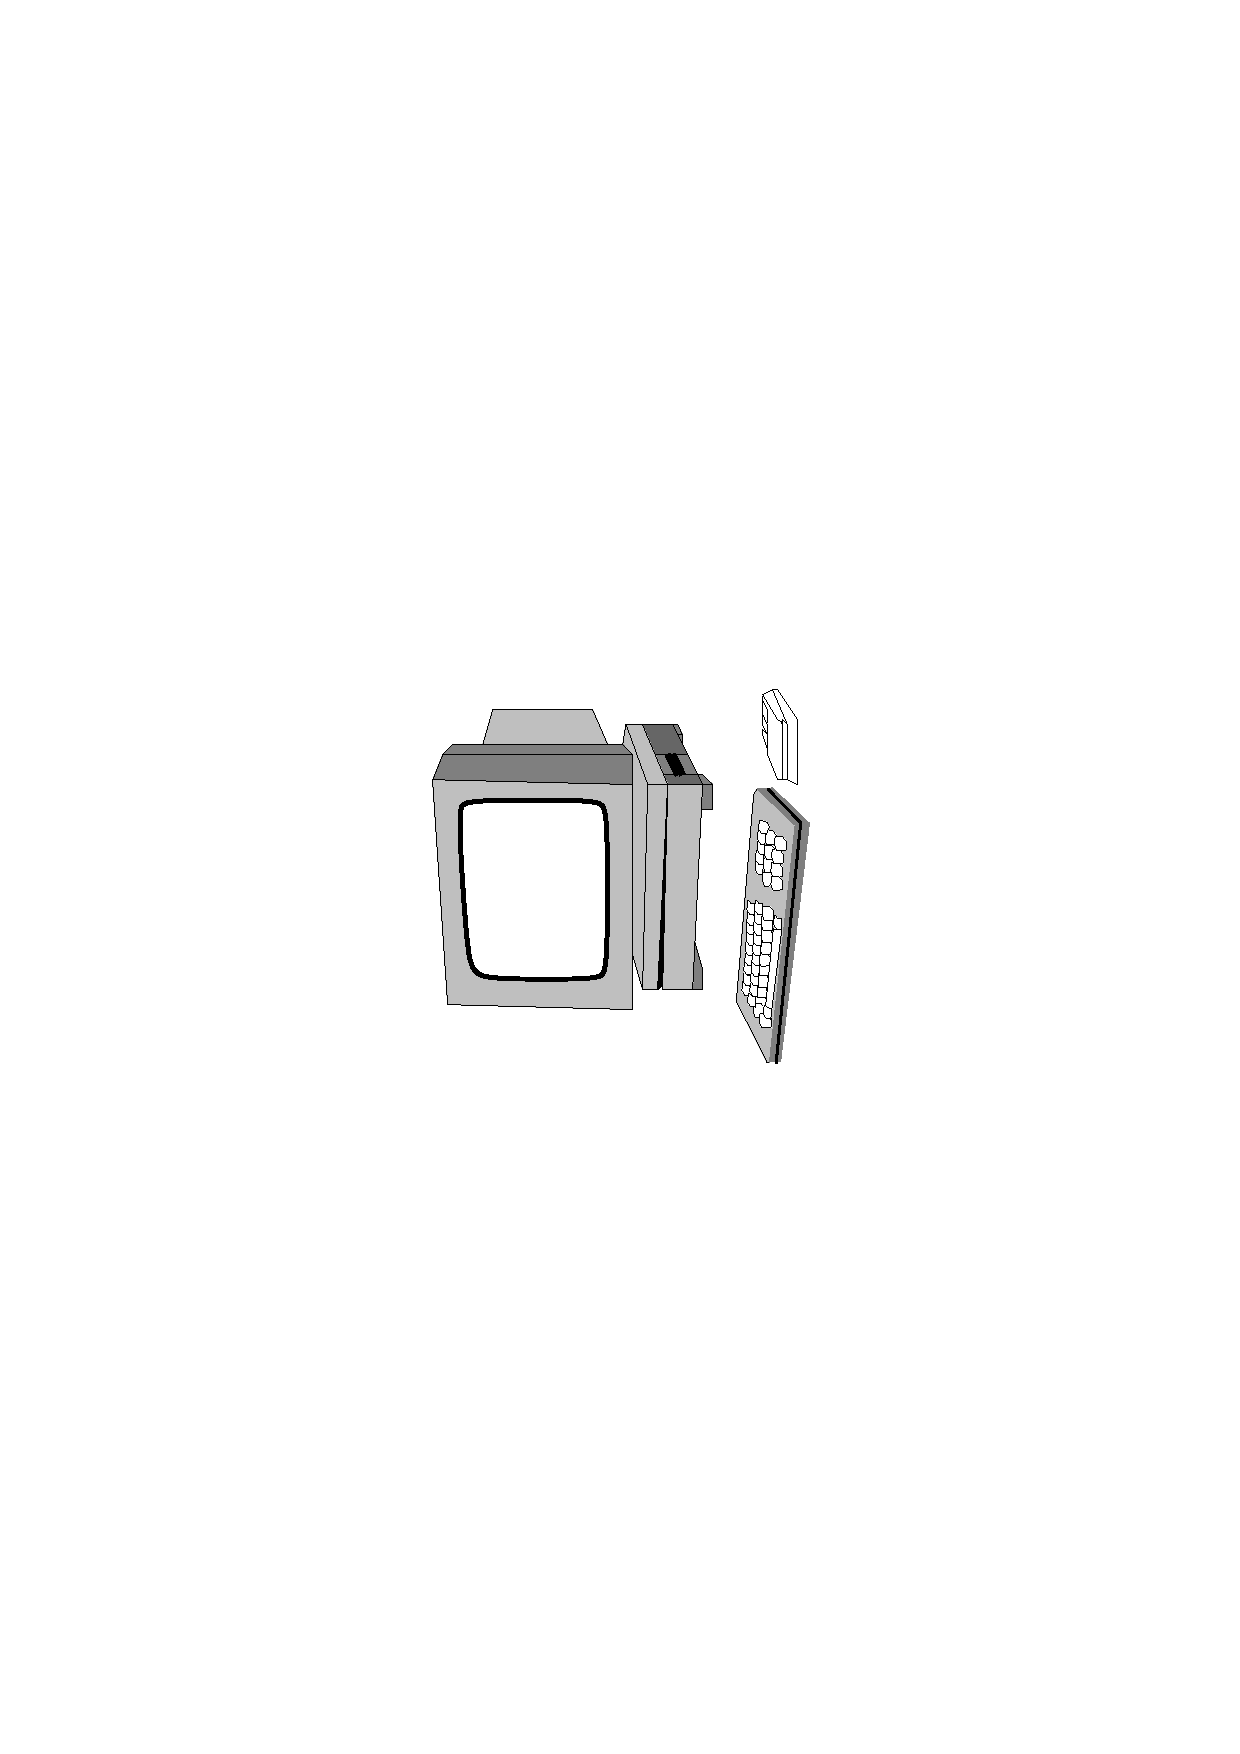
\includegraphics[width=4cm]{images/esempio}
   \caption{Esempio di figura\label{miafigura}}
   \end{figure}

\section{Equazioni}
   Le equazioni sono facilmente ottenibili, per esempio
   osservate nel sorgente $f(x)=x^{2}_{ij}\times \frac{(x+2)}{4}$
   oppure il suo equivalente~\ref{myeq} ottenuto utilizzando l'ambiente
   \emph{equation}:

   \begin{equation}
   \lim_{n \to \infty}
   \sum_{k=1}^n \frac{1}{k^2}
   = \frac{\pi^2}{6}
   \label{myeq}
   \end{equation}

\section{Lettere accentate\label{accenti}}

   Il \LaTeX2\/
   le gestisce benissimo: àèìòùÀÈÌÒÙáéíóúÁÉÍÓÚ (se avete l'accortezza di salvare i file con codifica \texttt{UTF-8}
   ma le nostre tastiere un po' meno\footnote{in realt\`a a volte l'ALT di destra
   usato con la vocale opportuna o il tasto sopra/sottostante (con eventualmente lo
   shift per le maiuscole) produce i vari tipi di accento (acuto, ottuso, dieresi\ldots).},
   allora in questo caso si usa:
   \`a\`e\`{\i}\`o\`u\`A\`E\aa\v e e cos\`{\i} via...
   \newpage
   Comunque per avere maggiori informazioni leggetevi la guida \emph{The Not So Short Introduction to \LaTeX2}
   che trovate già stampata da qualche parte nei laboratori.

\chapter{La Bibliografia}

   Per la gestione semplice e intuitiva della bibliografia si usa un programma
   aggiuntivo, il \BibTeX. A tal fine provate a dare il comando
   \texttt{bibtex tesi} e poi ri-latexxare due volte\footnote{se non funziona
   probabilmente non vi siete copiati i file local.bib e public.bib.}.
   Usando xdvi potrete notare che \`e stata completata la bibliografia
   e inserite le seguenti citazioni~\cite{sql,cv1,itsc99,mpi-boselli,mpipov,isata99,spie99,ipps99,iv98-1,iv98-2,spie98,isata97,iv97,camp97,canpc,ica3pp97,eusipco96,iv96,icip96}

   Per capire come \`e stato ottenuto il tutto guardate il sorgente, 
   provate poi ad osservare i file .bib per capire come aggiungere materiale da
   citare (il tutto \`e comunque spiegato in~\cite{btxdoc})\footnote{In realt\`a
   \`e decisamente conveniente includere file di bibliografie gi\`a esistenti.
   Per esempio,
   la maggioranza di voi hanno gi\`a definita una variabile BIBINPUTS che punta, tra le altre cose, ad
   alcune directory dove esistono alcuni file .bib che \`e gi\`a possible
   includere. Sicuramente il vostro co/relatore ha una directory in cui sono contenuti
   uno o pi\`u file .bib con le citazioni che fanno al vostro caso, fatevela dire
   e modificate la variabile di ambiente BIBINPUTS (nel file .user-cshrc) aggiungendo
   il \emph{path} opportuno.}

   Dal nostro sito web (area studenti) è possibile scaricarsi il database in formato \BibTeX di
   tutte le tesi sperimentali dal 1990 ai giorni nostri.




      \chapter{Controllo dei Robot}

Questo capitolo tratta tutte le nozioni e accorgimenti utillizzati per la creazione del nodo di comunicazione con i robot e-Puck
\section{Comunicazione}
	Come gi\`a anticipato nel capitolo precedente, la comunicazione con i robot avviene tramite una connessione seriale virtuale attraverso la quale vengono scambiati messaggi sotto forma di array di caratteri.
	
	Il firmware precaricato negli e-Puck fornisce una modalit\`a di interazione tramite connessione seriale nella quale \`e possibile accedere ai valori misurati da tutti i sensori e impartire vari comandi.
	In particolare inviando ``D,\emph{fl},\emph{fr}\textbackslash n'' \`e possibile impostare la frequenza di passo dei motori sinistro e destro rispettivamente ai valori di \emph{fl} e \emph{fr}.
	I valori accettabili per le due frequenze sono i numeri interi compresi tra -1000 e 1000, frequenze alle quali corrisponde una rotazione completa indietro o avanti della ruota in un secondo.
	
	  
\section{Modellizzazione}
	I robot utilizzati possono essere classificati come dei monocicli ad azionamento differenziale, l'assenza di una rotella di suppporto non crea problemi in quanto lo scheletro del robot permette la stabilit\`a e consente il movimento.
	\begin{figure}[H]
	\centering
	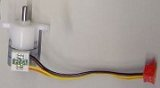
\includegraphics[width=4cm]{images/motor+cable}
	\caption{Modello schematico di un monociclo ad azionamento differenziale \label{unicycle}}
	\end{figure}
	
	Secondo questo modello il robot pu\`o avere due distinte componenti di velocit\`a: una di traslazione \emph{v}, ortogonale all'asse delle due ruote e parallela al piano di spostamento, e una di rotazione $\omega$ ortogonale al piano di spostamento del robot nel punto medio della distanza tra le due ruote.
	
	Da \emph{v} e $\omega$ possono essere stabilite le velocit\`a da assegnare alle singole ruote $\omega$r e $\omega$l tramite le seguenti relazioni in cui r \`e il raggio delle ruote e d la distanza tra i centri delle ruote:
	
	\begin{center}		
	\begin{tabular}{ccc}
			$\bigg \{
				\begin{array}{r}
				v=\frac{(\omega r+\omega l)r}{2}\\
				\omega = \frac{(\omega r-\omega l)r}{d}\\
				\end{array}$ 
 	& $\to$
 	&$\bigg \{
 		\begin{array}{r}
 		\omega r=\frac{2\emph{v}+d\omega }{r}\\
 		\omega l= \frac{2\emph{v}-d\omega}{r}\\
 		\end{array}$   \\ 
	\end{tabular} 
	\end{center}
	
	
	Per ricavare la frequenza di passo delle ruote si moltiplica i valori ottenuti per  $\frac{1000}{2\pi}$ che corrisponde al rapporto tra il numero di passi necessari per compiere una rotazione completa della ruota e una rotazione completa in radanti.
	
	\begin{center}	
	$\begin{array}{r}
	 		fr=\frac{1000}{2\pi}\times \omega r\\ 
	 		fl= \frac{1000}{2\pi}\times \omega l\\
	 		\end{array}$
	\end{center}
	
	Il nodo realizzato dunque riceve un messaggio tramite topic contenente \emph{v} e $\omega$ e ricava le frequenze di passo da assegnare alle ruote.
	Questi valori sono inviati al robot tramite connessione seriale utilizzando il messaggio descritto nella sezione precedente.
	Inoltre se il nodo non riceve messaggi di velocit\`a per due secondi invia al robot un comando per fermare le ruote ovvero imposta la frequenza di passo delle ruote a 0.
	
\section{Accorgimenti}
	Per evitare eventuali problemi di connessione e assicurare che le connessioni siano ripartite correttamente tra i due adatatori Bluetooth \`e stato creato uno script con linguaggio bash che utilizza i comandi ``rfcomm release'' e ``rfcomm bind'' per associare a ogni adattatore quattro robot tramite gli indirizzi MAC dei vari dispositivi.
	Lo script viene lanciato digitando ``./epuckbtset.sh'' in un terminale che punta alla cartella contenente il file bash.
	 	
	



      \chapter{Odometria}
	La soluzione utilizzata per rilevare la posizione dei robot all'interno dell'arena include l'utilizzo di metodi di computer vision in grado di rilevare contemporaneamente sia la posizione che l'orientamento di marker grafici attraverso le immagini fornite dalla webcam.
	
	L'acquisizione delle immagini dalla fotocamera avviene tramite il nodo ROS \emph{usb\_cam} che comunica con il sensore di immagini utilizzando il protocollo V4L (video for linux) e pubblica i fotogrammi ottenuti tramite \emph{image\_transport}, il protocollo standard per la trasmissione delle immagini in ROS.

\section{Calibrazione della fotocamera}
	Per riconoscere in maniera ottimale i marker l'immagine proveniente dalla fotocamera deve essere rettificata per bilanciare la distorsione introdotta dalle lenti.
	
	Per ottenere una rettificazione ottimale \`e necessario generare il file di calibrazione della fotocamera, questo file \`e ottenuto utilizzando l'applicazione ROS \emph{camera\_calibration} che calcola i parametri di distorsione.
	
	La procedura di calibrazione implica l'utilizzo di una scacchiera con dimensioni ben definite
	\begin{figure}[H]
	\centering
	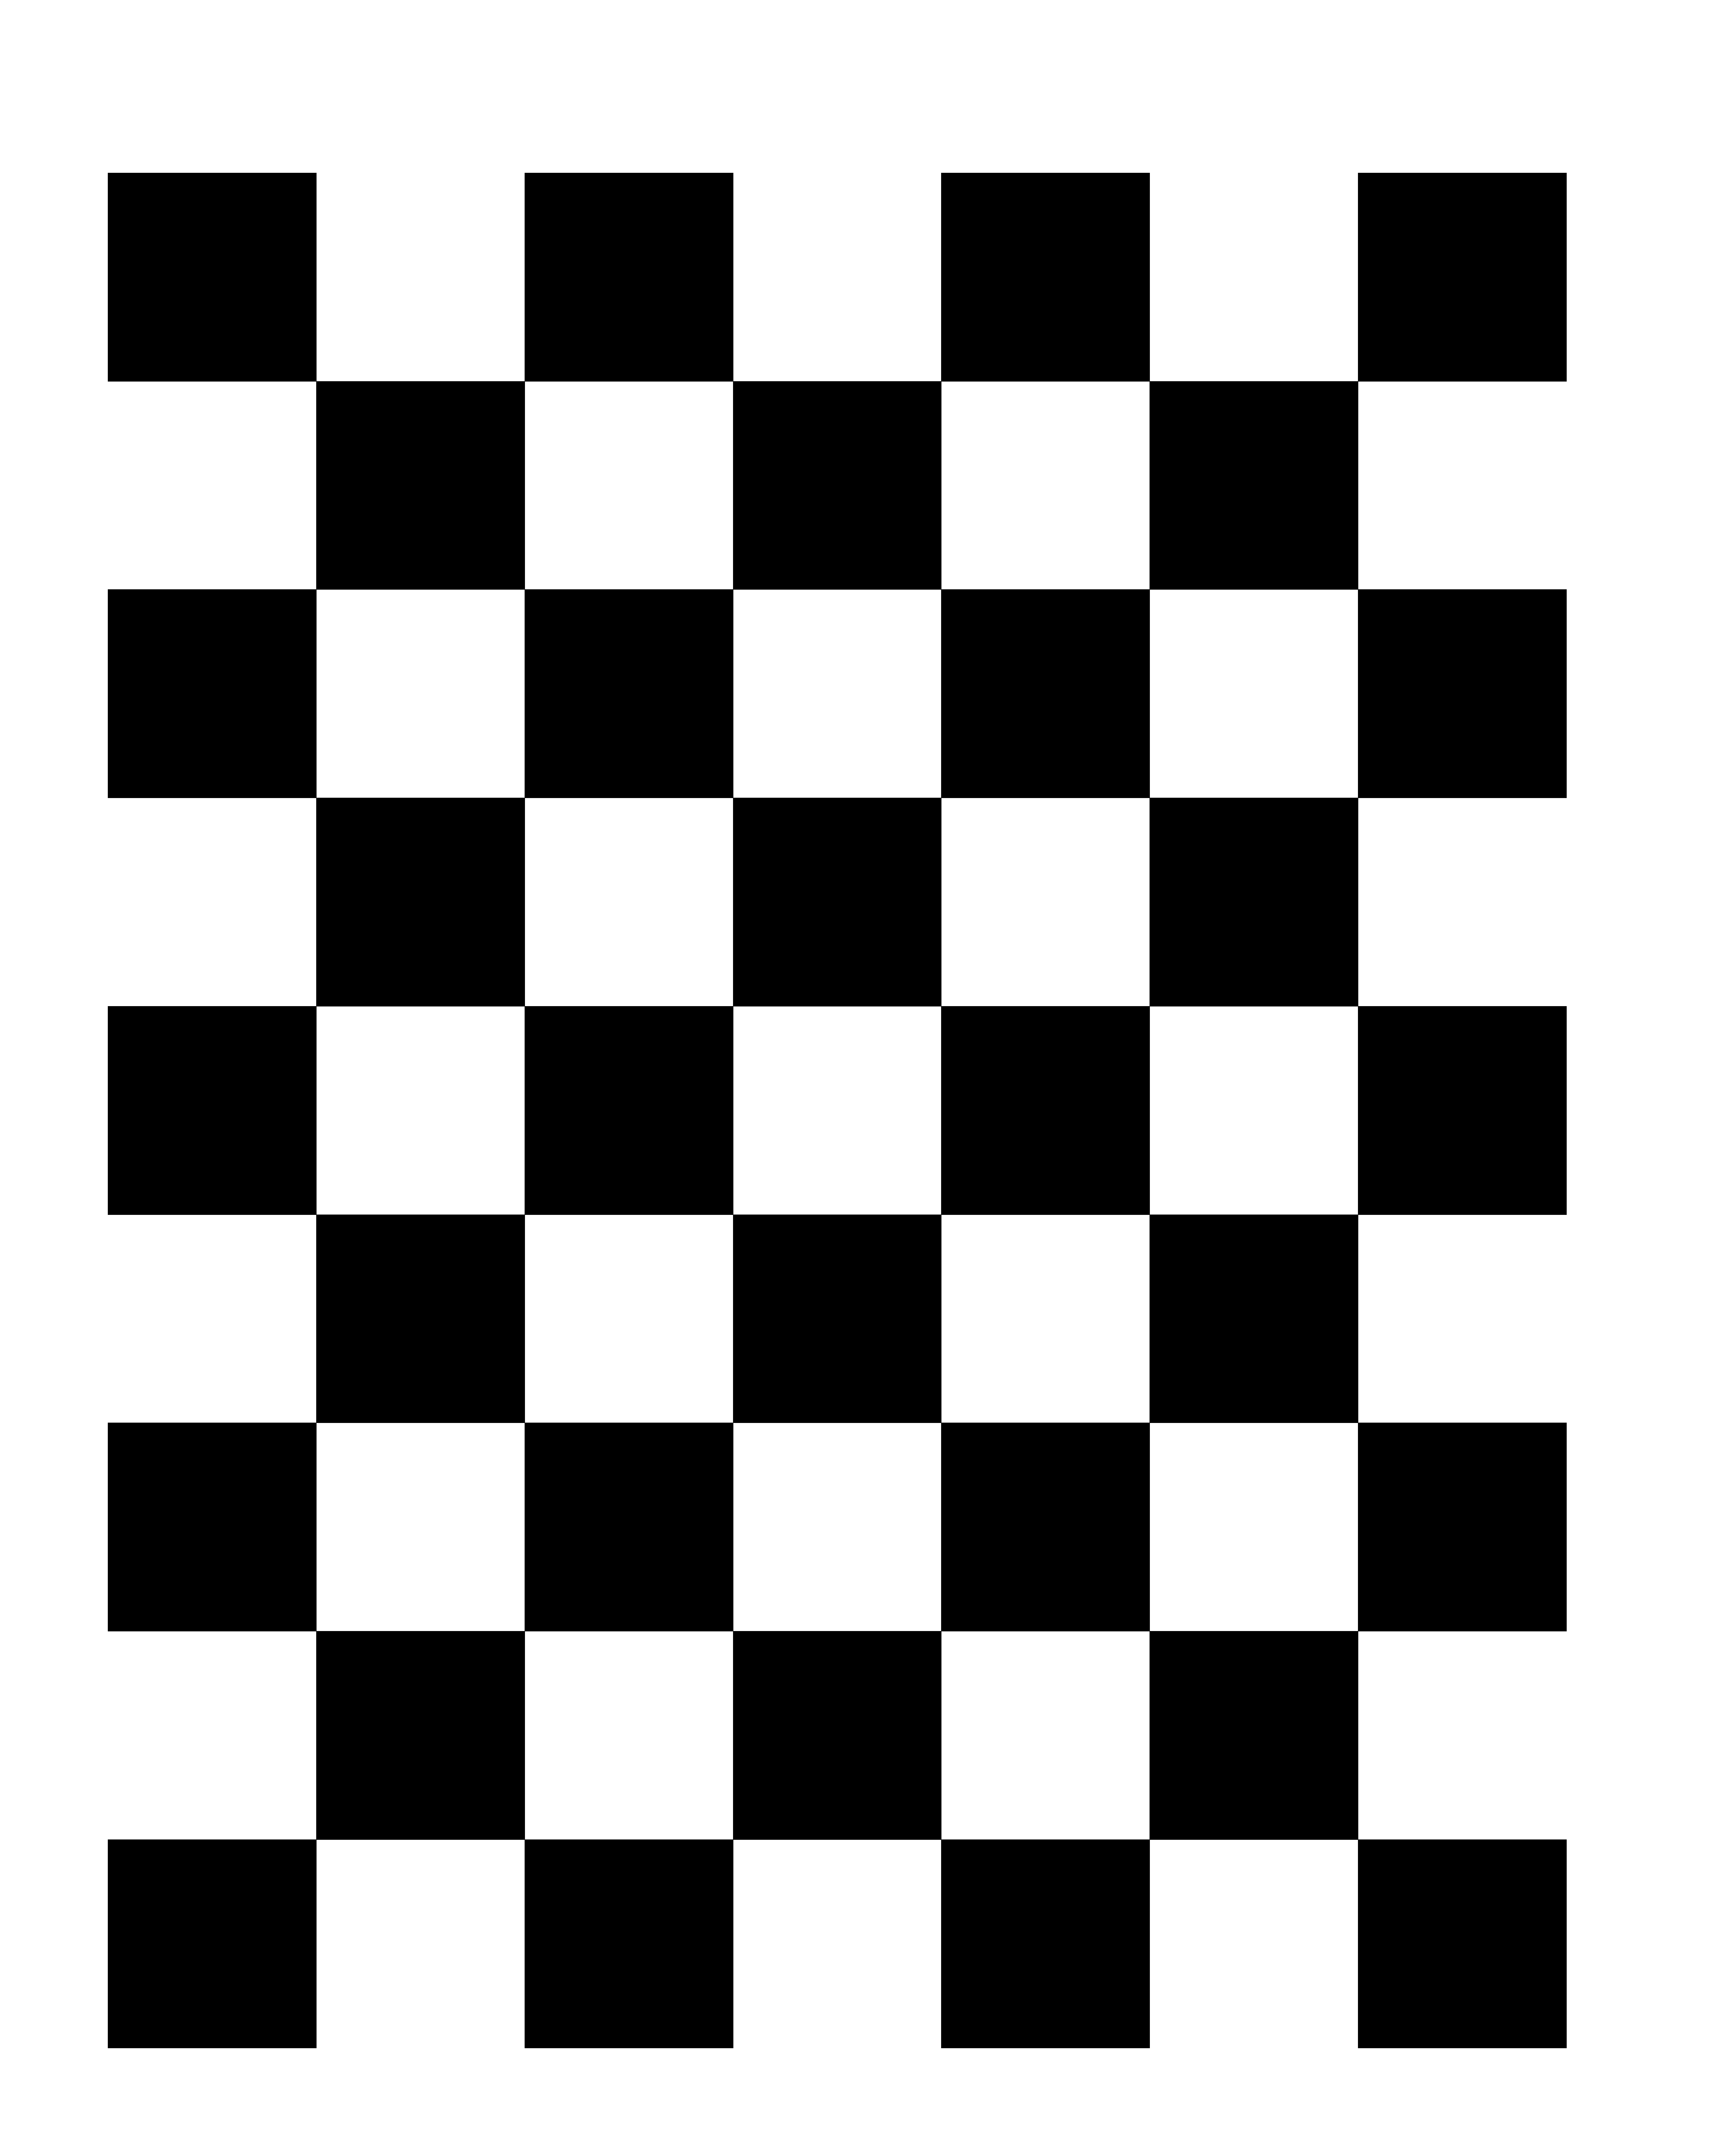
\includegraphics[width=0.4\linewidth, angle=90]{./images/check-108}
	\caption{Scacchiera 8 x 6}
	\label{fig:check-108}
	\end{figure}

	Una volta avviata l'applicazione si procede all'acquisizione dei dati traslando e ruotando la scacchiera lungo l'intero campo visivo della fotocamera fino a quando il software non comunica di aver acquisito sufficienti informazioni per la calibrazione. Il software ora pu\`o calcolare i dati di calibrazione e salvarli in un file formato YAML.
	
	La vera rettificazione dell'immagine avviene attraverso il nodo \emph{image\_proc} che processa l'immagine utilizzando i dati di calibrazione e restituisce l'immagine rettificata sempre utilizzando il protocollo di trasmissione di immagini di ROS.
	\huge
	 \emph{inserire immagini di esempio immagini rettificate e non}
	 \normalsize
	 
\section{Software di riconoscimento: ArUco}
	
\subsection{Markers}
\subsection{Boards}
\section{Compatibilit\`a con ROS}
\subsection{TF}
      \chapter{Controllo in Formazione e Teleoperazione}
\section{Formazione}
\section{Teleoperazione}

% da qui in poi \chapter genera un'appendice
\appendix
\renewcommand{\chaptermark}[1]{\markboth{{\appendixname}\ \thechapter.\hspace{1em}#1}{}}

      \chapter{Esempio di appendice}


Un po' di testo per generare x pagine.


DE:  The Soviets seem to have difficulty implementing modern technology.
     Would you comment on that?

Belenko:  Well, let's talk about aircraft engine lifetime.  When I flew the
          MiG-25, its engines had a total lifetime of 250 hours.

DE:  Is that mean-time-between-failure?

Belenko:  No, the engine is finished; it is scrapped.

DE:  You mean they pull it out and throw it away, not even overhauling it?

Belenko:  That is correct.  Overhaul is too expensive.

DE:  That is absurdly low by free world standards.

Belenko:  I know.
DE:  The Soviets seem to have difficulty implementing modern technology.
     Would you comment on that?

Belenko:  Well, let's talk about aircraft engine lifetime.  When I flew the
          MiG-25, its engines had a total lifetime of 250 hours.

DE:  Is that mean-time-between-failure?

Belenko:  No, the engine is finished; it is scrapped.

DE:  You mean they pull it out and throw it away, not even overhauling it?

Belenko:  That is correct.  Overhaul is too expensive.

DE:  That is absurdly low by free world standards.

Belenko:  I know.
DE:  The Soviets seem to have difficulty implementing modern technology.
     Would you comment on that?

Belenko:  Well, let's talk about aircraft engine lifetime.  When I flew the
          MiG-25, its engines had a total lifetime of 250 hours.

DE:  Is that mean-time-between-failure?

Belenko:  No, the engine is finished; it is scrapped.

DE:  You mean they pull it out and throw it away, not even overhauling it?

Belenko:  That is correct.  Overhaul is too expensive.

DE:  That is absurdly low by free world standards.

Belenko:  I know.
DE:  The Soviets seem to have difficulty implementing modern technology.
     Would you comment on that?

Belenko:  Well, let's talk about aircraft engine lifetime.  When I flew the
          MiG-25, its engines had a total lifetime of 250 hours.

DE:  Is that mean-time-between-failure?

Belenko:  No, the engine is finished; it is scrapped.

DE:  You mean they pull it out and throw it away, not even overhauling it?

Belenko:  That is correct.  Overhaul is too expensive.

DE:  That is absurdly low by free world standards.

Belenko:  I know.
DE:  The Soviets seem to have difficulty implementing modern technology.
     Would you comment on that?

Belenko:  Well, let's talk about aircraft engine lifetime.  When I flew the
          MiG-25, its engines had a total lifetime of 250 hours.

DE:  Is that mean-time-between-failure?

Belenko:  No, the engine is finished; it is scrapped.

DE:  You mean they pull it out and throw it away, not even overhauling it?

Belenko:  That is correct.  Overhaul is too expensive.

DE:  That is absurdly low by free world standards.

Belenko:  I know.



çççç çç çç aççe


\clearpage
\addcontentsline{toc}{chapter}{Bibliografia}
\bibliographystyle{abbrv}
\bibliography{tesid,public} % ATTENZIONE se
                            % non avete la variabile di ambiente BIBINPUTS
                            % correttamente impostata non vi trova tesid.bib !!

\cfoot{\emph{Finito di stampare il \today\/ utilizzando \LaTeXe}}
\end{document}





















